
%(BEGIN_QUESTION)
% Copyright 2006, Tony R. Kuphaldt, released under the Creative Commons Attribution License (v 1.0)
% This means you may do almost anything with this work of mine, so long as you give me proper credit

Shown here is the response of a proportional+derivative controller to a ramping process variable (with a constant setpoint).  Calculate the controller's proportional and derivative constant settings, based on what you see in the graph.  Also, determine whether this controller is direct or reverse acting, and mark the features of the output plot corresponding to proportional action and to derivative action.

$$\includegraphics[width=15.5cm]{i01543x01.eps}$$

The time scale on the chart is minutes:seconds.

\underbar{file i01543}
%(END_QUESTION)





%(BEGIN_ANSWER)

Controller action = {\it reverse}

\vskip 10pt

$K_p$ = 1

\vskip 10pt

$\tau_d$ = 1 minute = 60 seconds

\vskip 10pt

$$\includegraphics[width=15.5cm]{i01543x02.eps}$$

%(END_ANSWER)





%(BEGIN_NOTES)



%INDEX% Control, proportional + derivative: graphing controller response

%(END_NOTES)


